%!TEX root = ../main.tex

\chapter{Introduction}
\label{introduction}

Today's computing platforms are becoming increasingly complex with multiple interconnected computing nodes, each with multiple multicore CPU chips, and sometimes coupled with hardware accelerators. While the application performance is an important issue to tackle, the efficient usage of the resources of these systems is a crucial subject that needs to be addressed. Guaranteeing that the available computational resources are being fully used by an application may require deep knowledge of the underlying architecture details of both CPUs and hardware accelerators and extensive tuning of each individual application. It is important to understand the resources on a CPU, such as the computing units organisation, benefits and limitations of using multiple cores, and cache memory hierarchy, to avoid underusing the full computational potential of the device. The architecture design of many-core hardware accelerators have significant differences from device to device with no standard yet defined, unlike current CPUs. The programmer must know the architectural details of each hardware accelerator to produce efficient code. Moreover, the communications among the CPU and hardware accelerators must be managed by the programmer and may significantly affect the efficiency of an application.

From the hardware point of view, efficiency has a different meaning: engineers consider it to be the ratio between power usage and computational throughput. This is a subject of extensive research known as ``Green Computing'', where the goal is to reduce power consumption of the hardware with little impact to its performance. This is not only important for mobile computing but also to reduce the cost of maintaining huge computing clusters and data centres.

Computing clusters are the most popular High Performance Computing (HPC) platform and are constituted of many computing nodes, with possibly different characteristics, interconnected by specialised communication channels in a distributed memory environment. The computing nodes may be homogeneous or heterogeneous platforms, where the first has only one or more CPUs in a shared memory environment, and the latter has hardware accelerators connected by a PCI-Express interface to the CPUs, in a distributed memory environment. This means that the data is always visible to the CPUs, but must be explicitly transferred to the accelerator devices. The management of the data may affect the performance and efficiency of an application. Code parallelism is a must to take advantage of the multiple cores in both the CPUs and the hardware accelerators, with the programming model differing from shared to distributed memory environments. Data races, resource contention and, in heterogeneous systems, explicit memory transfers are complex issues that the programmer must tackle. Also, each accelerator manufacturer uses their own frameworks and compilers for programming their devices. With the current computational systems rapidly changing, scientists restrain from investing on academic formation in computer science, opting for self-learning these complex principles, and often avoid developing code for hardware accelerators. These factors reinforced the collaboration of multidisciplinary teams of scientists from various fields with computer scientists to develop high performing, efficient and robust applications.

The European Organization for Nuclear Research \cite{CERN} (CERN, acronym for \textit{Conseil Européen pour la Recherche Nucléaire}) is a consortium of 21 European countries, and more than 30 ``observer'' countries, with the purpose of operating the largest particle physics laboratory in the world. Founded in 1954, CERN is located in the border between France and Switzerland, and employs thousands of scientists and engineers representing 608 universities and research groups of 113 different nationalities.

CERN research focus on the basic constituents of matter to understand the fundamental structure of the universe, which started by studying the atomic nucleus but quickly progressed into high energy physics (HEP), namely on the interactions between particles. The instrumentation used in nuclear and particle physics research is essentially formed by particle accelerators and detectors, alongside with the facilities necessary for delivering the protons to the accelerators. The Large Hadron Collider (LHC) particle accelerator (later presented) speeds up groups of particles close to the speed of light, in opposite directions, inducing a controlled collision at the detectors core (the collision of two particles is referred as an ``event''). The detectors record various characteristics of the resultant particles of each collision, such as energy and momentum, which originate from complex decay processes of the original particles. The purpose of these experiments is to test models and predictions in High Energy Physics (HEP), such as the Standard Model, by confirming or discovering new particles and interactions.

CERN started with a small low energy particle accelerator, the Proton Synchrotron \cite{CERN:PS} inaugurated in 1959, but soon its equipment was iteratively upgraded and expanded. The current facilities are constituted by the older accelerators (some already decommissioned) and particle detectors, as well as the newer Large Hadron Collider (LHC) \cite{CERN:LHC} high energy particle accelerator, located 100 meter underground and with a 27 km circumference length. There are currently seven experiments running on the LHC: CMS \cite{CERN:CMS}, ATLAS \cite{CERN:ATLAS}, LHCb \cite{CERN:LHCb}, MoEDAL \cite{CERN:MoEDAL}, TOTEM \cite{CERN:TOTEM}, LHC-forward \cite{CERN:LHCf} and ALICE \cite{CERN:ALICE}. Each of these experiments have their own detector on the LHC and conduct HEP experiments, using distinct technologies and research approaches. One of the most relevant researches being conducted at CERN is the validation of the Standard Model and discovery of the Higgs boson theory. The ATLAS experiment, a key project at CERN, aims to study the properties of the recently discovered Higgs boson \cite{Higgs}, the search for new particles predicted by models of physics beyond the Standard Model like Susy, searches for new heavy gauge bosons and precision measurements where the top quark is of utmost importance. During the next year the LHC will be upgraded to increase its luminosity, e.g., the amount of energy of the accelerated particle beams.

Approximately 600 millions of collisions occur every second at the LHC. Particles produced in head-on proton collisions interact with the detectors of the ATLAS experiment, generating massive amounts of raw data as electric signals. It is estimated that all the detectors combined produce 25 petabytes of data per year \cite{CERN:DATA1,CERN:DATA2}. CERN does not have the financial resources to afford the computational power necessary to process all the data, which motivated the creation of the Worldwide LHC Computing Grid \cite{CERN:WLHCCG}, a distributed computing infrastructure that uses the resources of scientific community for data processing. The grid is organized in a hierarchy divided in 4 tiers. Each tier is made by one or more computing centres and has a set of specific tasks and services to perform, such as store, filter, refine and analyse all the data gathered at the LHC.

The Tier-0 is the data centre located at CERN. It provides 20\% of the total grid computing capacity, and its goal is to store and reconstruct the raw data gathered at the detectors in the LHC, converting it into meaningful information, usable by the remaining tiers. The data is received on a format designed for this reconstruction, with information about the event, detector and software diagnostics. The output of the reconstruction has two formats, the Event Summary Data (ESD) and the Analysis Object Data (AOD), each with different purposes, containing information of the reconstructed objects and calibration parameters, which can be used for early analysis. This tier distributes the raw data and the reconstructed output by the 11 Tier-1 computational centres, spread among the different member countries of CERN.

Tier-1 computational centres are responsible for storing a portion of the raw and reconstructed data and provide support to the grid. In this tier, the reconstructed data suffers more reprocessing, refining and filtering the relevant information and reducing the size of the data, now in Derived Physics Data (DPD) format, then transferred to the Tier-2 computational centres. The size of the data for an event is reduced from 3 MB (raw) to 10 kB (DPD). This tier also stores the output of the simulations performed at Tier-2. The Tier-0 centre is connected to the 11 Tier-1 centres by high bandwidth optical fiber links, which form the LHC Optical Private Network.

There are roughly 140 Tier-2 computational centres spread around the world. Their main purpose is to perform both Monte-Carlo simulations and a portion of the events reconstructions, with the data received from the Tier-1 centres. The Tier-3 centres range from university clusters to small personal computers, and they perform most of the events reconstruction and final data analysis. In the CERN terminology, an analysis is the denomination of an application which is designed to process a given amount of data in order to extract relevant physics information about events that may support a specific HEP theory.

These factors enforce the need to process more data, more accurately, in less time, which often leads to investments on larger computing clusters to improve the quality of the research results. However, most scientific code was not designed and/or developed for an efficient use of the available computational resources. If these applications were adequately designed (or tuned), the event analysis throughput could be massively increased. An efficient parallel application can significantly improve its performance at a much lower cost \cite{Msc:AMP}.

The Laboratório de Instrumentação e Física Experimental de Partículas (LIP) \cite{LIP} is a portuguese scientific and technical association for research on experimental high energy physics and associated instrumentation. LIP has a strong collaboration with CERN as it was the first scientific organization from Portugal that joined CERN, in 1986. It has laboratories in Lisbon, Coimbra and Minho and 170 people employed. LIP researchers have produced several applications for testing at ATLAS several HEP theoretical models that use Tier-3 computational resources for data analysis. Most of the analysis applications use in-house developed skeleton libraries, such as the LipCbrAnalysis and LipMiniAnalysis.

\section{Motivation, Goals, and Scientific Contribution}
\label{motivation}

With an increase in particle collisions and data being produced by the detectors at the LHC, research groups will need a larger budget to acquire and maintain the required computational resources to keep up with the analysis. Adding to this increase, research groups working on the same experiment enforce positive competition to find and publish relevant results. The amount and quality of event processing has a direct impact on the research, meaning that groups with more efficient computational resources become ahead of the competition.

Better physics are not only obtained by increasing the amount of events analysed; it is important to take into account the quality of each event analysis. Due to several intrinsic ATLAS experimental effects like energy and transverse momentum resolutions, the measured kinematic properties of particles produced in a collision, may be shifted within a range of $\pm1\%$, implying an intrinsic uncertainty which is propagated through the event analysis. It is possible to improve the reconstruction quality by varying the values measured by the detector within the said range, but with a significant impact to the analysis execution time, requiring a trade-off between the event processing throughput and their reconstruction quality.

To aid the development of these data analysis applications, scientists at LIP created a skeleton library named LipCbrAnalysis. It contains a set of physics utilities, such as specific classes and functions, and removes the need to code the input file reading, memory allocation of each event data, and output creation. With this, the programmer only needs to code the specific bits of the analysis filtering and reconstruction of events. An iteration of this skeleton was developed, named LipMiniAnalysis, with the purpose of reading a new structure of the input data files, and stripping the former skeleton of outdated features.

An efficiency study and optimisation of one of LIP production data analysis, used also as case study for some preliminary studies of this PhD pre-thesis work, was presented in \cite{Msc:AMP,paperAMP}. It tackled the computational inefficiencies on both homogeneous and heterogeneous platforms, and identified several limitations to performance scalability, specially when using hardware accelerators. The data analysis case study and the limitations identified with the LipMiniAnalysis skeleton are presented in subsection \ref{ttH}.

Dealing with scientific code is no trivial task due to the code structure and organization. Several studies \cite{SC:Nature,SC:Develop,SC:SC11,SC:28280} identified the causes that lead scientists to produce poor code:

\begin{center}
	\begin{itemize}
		\item Most scientists are self-taught programmers with no computer science background;
		\item Scientists disregard software engineering principals to produce long lasting, extendible, and efficient code;
		\item Scientists often iterate through the same application, producing legacy code (some applications currently in production are iterated on for the last 20 years), and not documenting it so that it can be used by others;
		\item Scientists usually are not aware of profiling and debugging tools, as well as parallelisation paradigms;
		\item Scientists do not understand the architectural details of computing systems, reducing the portability of the code they produce.
	\end{itemize}
\end{center}

To improve the quality of the scientific code, scientists agree that it is important to create an interface between their field and computer science by having multidisciplinary teams. However, computer scientists often lack the scientific knowledge required to be acknowledge as an integral part of these teams.Also, scientists are often sceptical to let others restructure, and even develop from scratch, legacy code that they are using for years.

\subsection{The Top Quark and Higgs Boson Decay}
\label{ttH}

At the LHC, two proton beams are accelerated close to the speed of light in opposite directions, set to collide inside a specific particle detector. This head-on collision triggers a chain reaction of decaying particles, and most of the final particles interact with the detector, allowing to record relevant data. One of the searches being conducted at the ATLAS Experiment relates to the study of the top quark and Higgs boson couplings. Figure \ref{fig:ttH} represents the final state topology of the associated production of two top quarks and one Higgs boson (that decays to two b-quarks), labelled from now on as \ttH production. Figure \ref{fig:ttbar} provides a schematic representation of the system to highlight certain features, such as the bottom quarks being jets of particles, and the leptons (both $l^+$ and $l^-$) being a muon and electron in the $t$ and $\bar{t}$ decays, respectively.

\begin{figure}[!htp]
	\begin{center}
		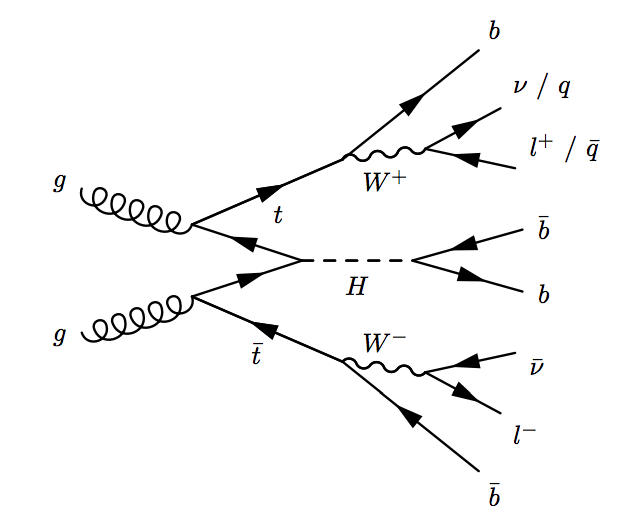
\includegraphics[scale=0.3]{imgs/ttH_feynman.png}
		\caption{Feynman diagram of the \ttbar and Higgs boson production.}
		\label{fig:ttH}
	\end{center}
\end{figure}

\begin{figure}[!htp]
	\begin{center}
		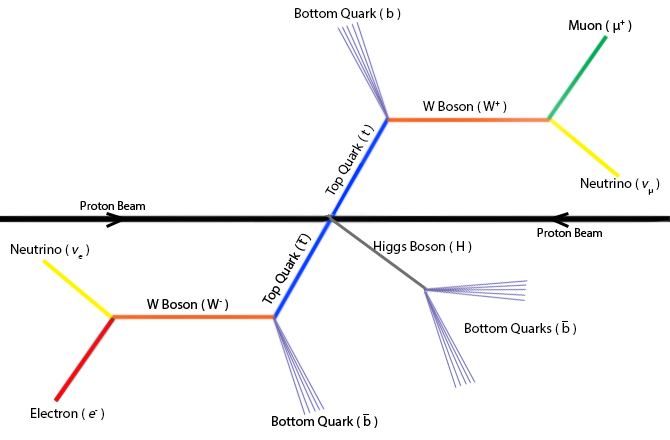
\includegraphics[scale=0.45]{imgs/ttbar_higgs.png}
		\caption{Schematic representation of the \ttbar system and Higgs boson decay.}
		\label{fig:ttbar}
	\end{center}
\end{figure}

Neutrinos do not interact with the detector, so their characteristics are not recorded. Since the top quark reconstruction requires the neutrinos, their characteristics are analytically determined with the known information of the system, through a kinematical reconstruction. However, the \ttbar system may not have a possible reconstruction: the reconstruction has an intrinsic uncertainty associated which determines its accuracy.

The amount of jets from bottom quarks and leptons present in the events may vary according to the decay channel of the $W$ bosons produced in the top quark decays. As shown in figure \ref{fig:ttbar}, four jets and two leptons are required to be present in the events. Two of the jets, together with two leptons are required to reconstruct the \ttbar system, and the remaining two jets are used for the Higgs boson reconstruction. For the kinematical reconstruction, every possible combination of jets and leptons must be evaluated and only the most accurate reconstruction of each event is considered. In a first step, the \ttbar system reconstruction is tried.  If it has a possible solution, the Higgs boson is reconstructed from the jets of the two remaining bottom quarks. The Higgs reconstruction does not use the jets which were associated to the best \ttbar system reconstruction. The overall quality of the event processing depends on the quality of both reconstructions.

For the global event reconstruction, several solutions can be tested if we assume that the ATLAS detector has an experimental energy-momentum resolution of $\pm1\%$, by varying these quantities within their uncertainty. This uncertainty is propagated into the \ttbar system and Higgs reconstructions, affecting their accuracy. To improve the quality of the reconstructions several random variations are applied to the measured values, within a maximum range of $|1\%|$ next to the measured values. The quality of the reconstructions and the application execution time is directly proportional to the amount of variations performed per combination. The goal is to do as many variations as possible within a reasonable time frame.

\begin{figure}[!htp]
	\begin{center}
		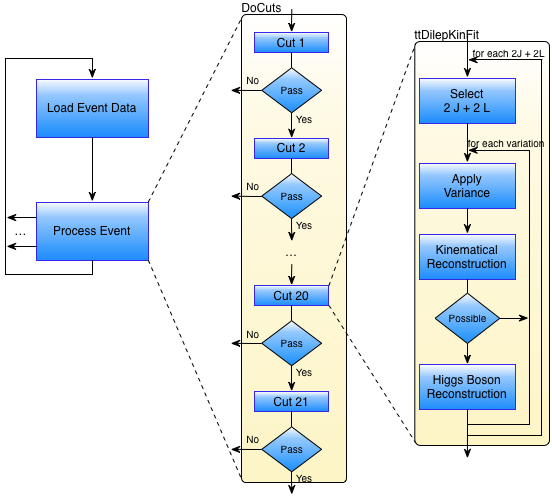
\includegraphics[scale=0.5]{imgs/graf_abstract_flow_with_kinfit.png}
		\caption{Schematic representation for the \tth application flow.}
		\label{fig:flow}
	\end{center}
\end{figure}

To reconstruct the \ttH system a data analysis application was developed, the \tth. The application flow is presented in figure \ref{fig:flow}. Each event data on an input file is individually loaded into a single global state, shared between the data analysis code and the LipMiniAnalysis, and it is overwritten every time a new event is loaded. The event is then submitted to a series of cuts, which filters events that are not suited for reconstruction. When an event reaches the cut 20, the \ttbar system and Higgs boson are reconstructed in the function \ttDilepKinFit, which is expected to be the most computing demanding. If the \ttbar system reconstruction fails, the current combination is discarded and the next is processed. If an event has a possible reconstruction it passes the final cut and its final information is stored.

\subsection{Goals and Scientific Contribution}
\label{goals}

\itodo{O que pode ser considerado no contexto da framework e compatibilidade com legacy code?}


